
\section{Datatset}
\label{sec:dataset}
Particular attention is needed in the construction of a good training dataset, 
in fact, as seen before in (\ref{subsec:supervised-learnig}), we deal with a 
supervised learning where we know the response of our labels and bounding box position's objects.
A script is provided that can build a dataset divided into folders: training, 
validation and testing; as you can see in figure \ref{fig:datasetstructure}.
A large number of figures per sample that clearly highlights the characteristics 
that you want to study allows a greater rate of success of the training 
preventing the \emph{overfitting}.
Acquiring a large number of images is not always achievable, using some 
augmentation techniques, virtually allows to increase the observability of a 
images, for example, by rotating, distorting and translating them.
The two train and validated folders are essential for the addition of the 
neural network.
Instead, the test folder contains a set of images that the network has never 
seen and so necessary to measure the degree of confidence acquired in the network.\linebreak
%
\begin{figure}[htb]
	\centering
	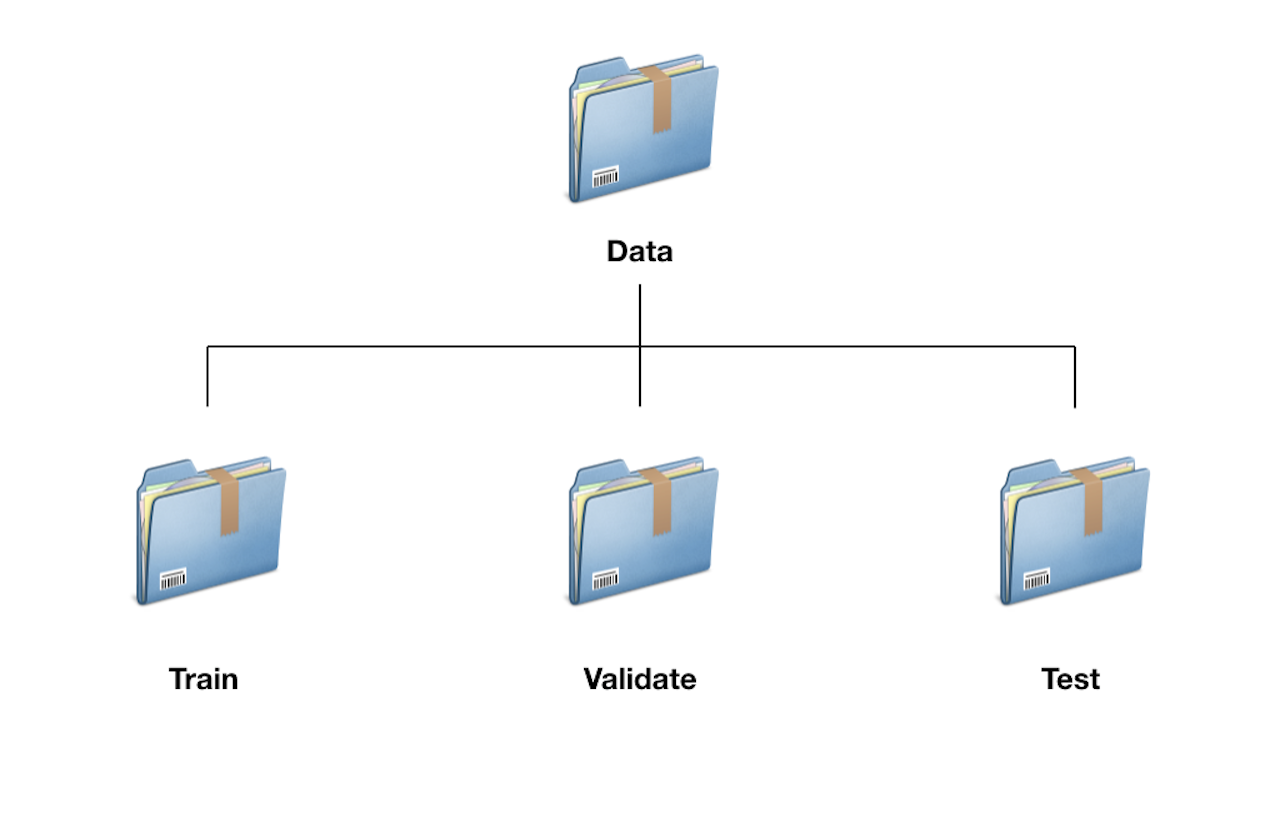
\includegraphics[width=0.75\textwidth]{structure.png}
	\caption{Dataset structure}
	\label{fig:datasetstructure}
\end{figure}
%
\subsection{Landing zone dataset}
\label{ssec:landing-zone}
%
The dataset was artificially constructed with a 3D Blender graphics program. 
The object of interest are the drone landing mats. These have different shapes
and colors in fact they are available in various color shapes. The signs on
these also vary from the classic H to X to more or less conspicuous symbols.
Thus three models were created, two with a circular plan and one with a square
plan. Textures were then applied to these two models to obtain a faithful
representation of that of concrete objects. After the construction of the carpet
models, it was necessary to contextualise them in credible scenarios. thus,
three main scenarios were created: a scenario placed in the middle of a road
junction. the second scenario near a straight road flanked by a sidewalk. the
third zone is set in the countryside. To take the shots, some photographic
factors were taken into account, in fact they are generated starting from the
technical characteristics of the Raspberry camera presented in section
(\ref{sec:raspicam}). Moreover, thanks to a simple script, the trigger points
were generated with respect to the landing mat position, these positions vary in
height, width and depth with respect to the carpet placed on the ground. A
scheme is visible in figures (\ref{fig:poi_dataset}).
%
\begin{figure}[!h]
	\centering
	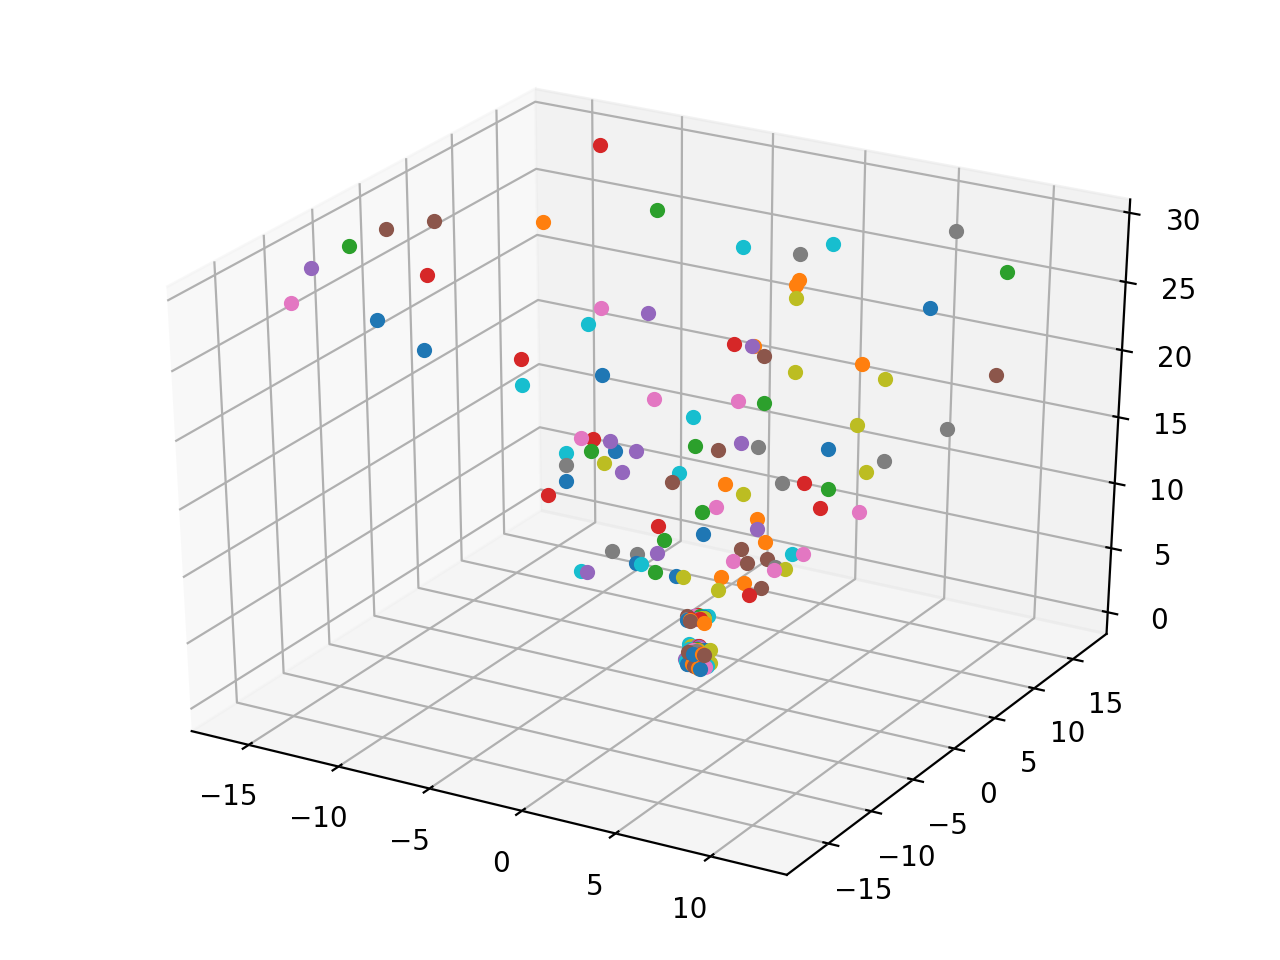
\includegraphics[width=0.75\textwidth]{poi_dataset.png}
	\caption{Configuration camera position.}
	\label{fig:poi_dataset}
\end{figure}

To increase the variety of rendered shots, a very basic day / night cycle was used to detect the color variation.
All the shots are taken with a top view as seen in the examples shown in 15666.





After completing the shots they annotated themselves highlighting the position
of the object of interest in the various shots and positions.
The process is carried out with the aid of a software that extracts and
generates the annotations. as shown in figure (\ref{fig:annotation}).
\begin{figure}[!h]
	\centering
	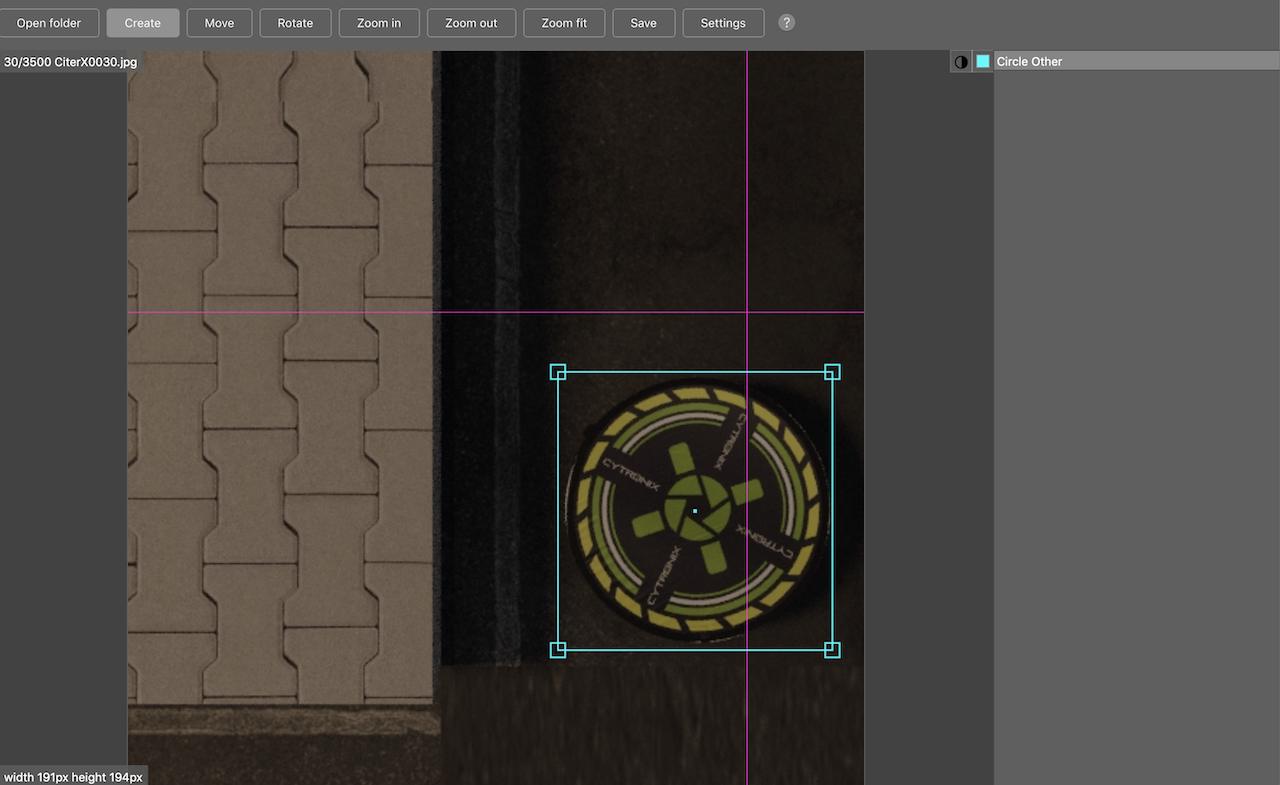
\includegraphics[width=0.75\textwidth]{annotation.png}
	\caption{Process of annotation.}
	\label{fig:annotation}
\end{figure}







\subsection{Thermal imaging dataset}
\label{ssec:thermal-image-dataset}